% !TeX program = pdflatex
\documentclass[border=6pt]{standalone}
\usepackage{tikz}
\usetikzlibrary{arrows.meta, positioning, calc}

\definecolor{MediumRed}{rgb}{0.925, 0.345, 0.345}
\definecolor{MediumGreen}{rgb}{0.37, 0.7, 0.66}
\definecolor{MediumBlue}{rgb}{0.015, 0.315, 0.45}
\definecolor{DarkBlue}{rgb}{0.05, 0.15, 0.35}

% s = cm por punto BLEU-4 ; r = separacion entre filas (cm)
\def\s{0.26}
\def\r{0.66}

\begin{document}
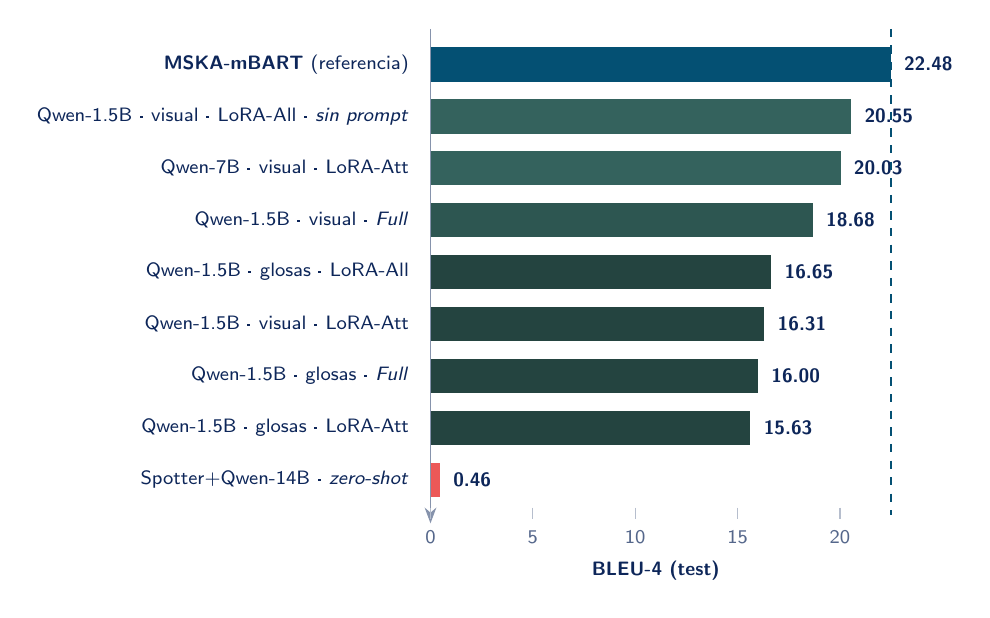
\begin{tikzpicture}[font=\sffamily]

\foreach \v/\lbl/\c [count=\i from 0] in {%
    22.48/{\textbf{MSKA-mBART} (referencia)}/MediumBlue,
    20.55/{Qwen-1.5B · visual · LoRA-All · \emph{sin prompt}}/MediumGreen!55!black,
    20.03/{Qwen-7B · visual · LoRA-Att}/MediumGreen!55!black,
    18.68/{Qwen-1.5B · visual · \emph{Full}}/MediumGreen!48!black,
    16.65/{Qwen-1.5B · glosas · LoRA-All}/MediumGreen!38!black,
    16.31/{Qwen-1.5B · visual · LoRA-Att}/MediumGreen!38!black,
    16.00/{Qwen-1.5B · glosas · \emph{Full}}/MediumGreen!38!black,
    15.63/{Qwen-1.5B · glosas · LoRA-Att}/MediumGreen!38!black,
    0.46/{Spotter+Qwen-14B · \emph{zero-shot}}/MediumRed}{%
    \fill[\c] (0, {-\i*\r-0.22}) rectangle ({\v*\s}, {-\i*\r+0.22});
    \node[anchor=west, font=\sffamily\scriptsize\bfseries, text=DarkBlue]
        at ({\v*\s}, {-\i*\r}) {\,\v};
    \node[anchor=east, font=\sffamily\scriptsize, text=DarkBlue]
        at (-0.15, {-\i*\r}) {\lbl};
}

% linea de referencia mBART
\draw[MediumBlue, dashed, thick] ({22.48*\s}, 0.45) -- ({22.48*\s}, {-8*\r-0.45});

% eje x
\draw[DarkBlue!50, -{Stealth[length=2mm]}] (0,0.45) -- (0,{-8*\r-0.55});
\foreach \x in {0,5,10,15,20}{
    \draw[DarkBlue!30] ({\x*\s},{-8*\r-0.35}) -- ({\x*\s},{-8*\r-0.5});
    \node[font=\sffamily\scriptsize, text=DarkBlue!70] at ({\x*\s},{-8*\r-0.72}) {\x};
}
\node[font=\sffamily\scriptsize\bfseries, text=DarkBlue] at ({11*\s},{-8*\r-1.15}) {BLEU-4 (test)};

\end{tikzpicture}
\end{document}
